\documentclass[onecolumn, draftclsnofoot,10pt, compsoc]{IEEEtran}
\usepackage{graphicx}
\usepackage{url}
\usepackage{setspace}
\usepackage{pgfgantt}
\usepackage{geometry}
\geometry{textheight=9.5in, textwidth=7in}

% 1. Fill in these details
\def \CapstoneTeamName{		Project LOOM}
\def \CapstoneTeamNumber{		36}
\def \GroupMemberOne{			William Selbie}
\def \GroupMemberTwo{			Trevor Swope}
\def \GroupMemberThree{			Luke Goertzen}
\def \CapstoneProjectName{		Project LOOM | Design an Internet of Things Rapid Prototyping System.}
\def \CapstoneSponsorCompany{	}
\def \CapstoneSponsorPerson{		Chet Udell}

% 2. Uncomment the appropriate line below so that the document type works
\def \DocType{	%Problem Statement
				Requirements Document
				%Technology Review
				%Design Documeet
				%Progress Report
				}
			
\newcommand{\NameSigPair}[1]{\par
\makebox[2.75in][r]{#1} \hfil 	\makebox[3.25in]{\makebox[2.25in]{\hrulefill} \hfill		\makebox[.75in]{\hrulefill}}
\par\vspace{-12pt} \textit{\tiny\noindent
\makebox[2.75in]{} \hfil		\makebox[3.25in]{\makebox[2.25in][r]{Signature} \hfill	\makebox[.75in][r]{Date}}}}
% 3. If the document is not to be signed, uncomment the RENEWcommand below
\renewcommand{\NameSigPair}[1]{#1}

%%%%%%%%%%%%%%%%%%%%%%%%%%%%%%%%%%%%%%%
\begin{document}
\begin{titlepage}
    \pagenumbering{gobble}
    \begin{singlespace}
        \hfill 
        % 4. If you have a logo, use this includegraphics command to put it on the coversheet.
        %\includegraphics[height=4cm]{CompanyLogo}   
        \par\vspace{.2in}
        \centering
        \scshape{
            \huge CS Capstone \DocType \par
            {\large\today}\par
            \vspace{.5in}
            \textbf{\Huge\CapstoneProjectName}\par
            \vfill
            {\large Prepared for}\par
            \Huge \CapstoneSponsorCompany\par
            \vspace{5pt}
            {\Large\NameSigPair{\CapstoneSponsorPerson}\par}
            {\large Prepared by }\par
            Group\CapstoneTeamNumber\par
            % 5. comment out the line below this one if you do not wish to name your team
            \CapstoneTeamName\par 
            \vspace{5pt}
            {\Large
                \NameSigPair{\GroupMemberOne}\par
                \NameSigPair{\GroupMemberTwo}\par
                \NameSigPair{\GroupMemberThree}\par
            }
            \vspace{20pt}
        }
        \begin{abstract}
% 6. Fill in your abstract    
			This client requirements document outlines the deliverables that the Computer Science Senior Capstone Group 36 will be producing and held accountable for - with regards to client satisfaction and Capstone course evaluation.
			The document addresses what the end result will be expected to do and be, but not how it is implemented. 
		\end{abstract}     
    \end{singlespace}
\end{titlepage}
\newpage
\pagenumbering{arabic}
\tableofcontents
% 7. uncomment this (if applicable). Consider adding a page break.
%\listoffigures
%\listoftables
\clearpage

% 8. now you write!
\section{Introduction}
	\subsection{Purpose}
	This document aims to define the goals, scope, requirements, and development direction of the software and firmware side of Project LOOM. This document does not address in depth the requirements of the hardware portions of Project LOOM. The focus is instead only on the scope of the project with regards to the work to be done by Computer Science Capstone Group 36. Additionally, this document explains what the system will be expected to do, not how it will do so. As such, some details of specific technologies, protocols, or hardware will be deferred to subsequent documents.While this document will present the dependencies of the project, with regards of what must be completed in order for others to begin, a specific timeline will not yet be provided. 
	This document is intended for the client of Project LOOM, Chet Udell, as well as the Senior Capstone course instructors to outline what can be expected of the Senior Capstone group to produce over the course of the project, and to provide a metric against which Group 36 will be evaluated.

	\subsection{Scope}
	With Project LOOM, we aim to create an open-source, plug-and-play, suite of modular building blocks, the extensible and easy programmability of which expands the demographic of people capable of implementing Internet of Things solutions. For users with limited technical expertise to create complex systems, we aim to build a system that abstracts out the more technical details, allowing them to focus on their system more than the implementation of the modules. The system should also be usable by higher level students and experts by allowing them to modify or write their own firmware, and create new modules. Project LOOM will be developed for university faculty demos of functionality, possible subsequent commercialization is currently outside of the scope of the Senior Capstone project.
	\subsection{Definitions, Acronyms, and Abbreviations}
	\textbf{The Internet of Things (IoT):} Entails an aggregate of systems (many embedded) capable of reading, transmitting, receiving, processing, and acting upon data. This often takes the form of a network of remotely connected devices that can be used for the purpose of autonomous data collection, or remote control and automation of various systems. \newline
	\textbf{Module:} An interchangeable, self-contained device that can be connected to an IoT network with minimal configuration. Connects to other modules to combine behaviors (i.e. a sensor attached to a WiFi adapter becomes a sensor that transfers data over WiFi). \newline
	\textbf{Gateway:} A wired or wireless node connecting multiple devices on a network (e.g. WiFi, Ethernet) \newline

	\subsection{References}
	\begin{enumerate}
		\item \textbf{Figure One:} \texttt{Gantt Chart}
		\item \textbf{Figure Two:} \texttt{License}
	\end{enumerate}
	
	\subsection{Overview}
	The remainder of this document will provide an overview of major functions of Project LOOM, followed by more specific information regarding these functions and constraints to their design, as well as characteristics of its users and the assumptions and dependencies that are inherent to its inception. A Gantt chart is provided to illustrate dependencies of the stages of the project.

\section{Overall Description}
	\subsection{Product Perspective}
	The scope of the work that Group 36 will be responsible for is a subset of that of the larger Project LOOM team. This subset includes the embedded firmware that will be run on the devices themselves, as well as the development of the graphical interface that will be used to program and monitor the connected devices.

		\subsubsection{User Interfaces}
		The main user interface will be presented via modules in MaxMSP that receive and process data in a readable way. Readability will be informally evaluated by whether or not faculty or other users are able to set up and understand the displays of program during our demos.
		
		\subsubsection{Software Interfaces}
		Project LOOM will interface with the following software in order to visualize data or to use the software as an output of the system:
			\begin{itemize}
				\item MaxMSP
				\item IFTTT
				\item Google Docs via PushingBox
				\item AdaFruit IO
				\item Plot.ly
				\item Anything else that accepts TCP/MQTT or UDP/OSC packetized data
			\end{itemize}
		
		\subsubsection{Hardware Interfaces}
		The following hardware interfaces (not necessarily exhaustive) will be used to make the modules. The construction itself is not a part of Group 36’s portion of Project LOOM:
		\begin{itemize}
			\item AdaFruit FeatherM0
			\item AdaFruit Feather32u4
			\item MPU6050
		\end{itemize}
		
	\subsection{Product Functions}
		The system must be able to:
		\begin{itemize}
			\item Receive and transmit data with physically and wirelessly connected modules.
			\item Perform actions based on received data.
			\item The firmware should be modular and configurable via a user interface.
		\end{itemize}
		Users must be able to:
		\begin{itemize}
			\item Select and visualize incoming sensor data on a network via MaxMSP
			\item Remotely trigger events on actuators and monitor these actions via a user interface
			\item Re-calibrate devices remotely
			\item Process or analyze this data for events, thresholds, feature recognition, remap to useful control signals
			\item Program the devices with the Arduino development environment by altering or replicating the open-source code on which the firmware is based
		\end{itemize}

	\subsection{User Characteristics}
	There are a range of possible users for the LOOM devices and software; the target audience is meant to span from novice hobbyists to experts. Anyone wanting to learn about or implement an IoT solution in a streamlined fashion should be able to pick it up out of the box and get a simple system working without any programming. On the other end of the spectrum, there are users with more technical expertise, who simply want well-designed sensors and actuators that work together in ways that make sense. Since Project LOOM is open-source, these users will be able to write their own software and firmware for the chips if they choose to do so.
	Project LOOM is currently being developed with the intent to be tested by university professors and their students.

	\subsection{Constraints}
		\textbf{Hardware Limitations:} The software must run on the following hardware: AdaFruit FeatherM0, AdaFruit Feather32u4, MPU6050i. \newline
		\textbf{Parallel Operation:} Sending and receiving should be possible at the same time, especially to and from any central computer. \newline
		\textbf{Reliability Requirements:} Will send notification if system has detected that a module is broken, offline, or otherwise less than functional. However, the project is not currently being held to any standards and reliability will not be quantified. \newline
		\textbf{Safety and Security:} Will be addressed to a reasonable effort, but not to the point that it restricts progress of the rest of the project. \newline
	
	\subsection{Assumptions and Dependencies}
	Our work will be built off of the framework of existing hardware and software of Project LOOM. We are assuming that our firmware and software will be run on functional hardware developed by a sister team of Project Loom. The firmware for the modules in Project LOOM will be developed with the Arduino development environment, and the interface for reading the data will be a plugin for MaxMSP.

\section{Specific Requirements}
	\subsection{External Interfaces}
	Inputs: 
	\begin{itemize}
		\item Open Sound Control packets giving instructions
		\item Commands from the gateway
		\item Requests for data
		\item Data from sensors
	\end{itemize}
	Outputs: 
	\begin{itemize}
		\item Actuator behavior (servos, motors, lights, etc.)
		\item Open Sound Control digital/analog 
		\item Data to the gateway
	\end{itemize}
	
	\subsection{Functions}
	Modules will each have their own functionality but should be able to connect to the software and network of other modules without difficulty. The user should be able to use software to view data reading or to cause behaviors of actuator modules via outputs. Software can be used to translate outputs from one module into a usable input to another module, or simply process and display the data for the user. A comprehensive list of modules intended to be developed is not yet defined.

	\subsection{Performance Requirements}
	There are not currently requirements regarding the speed of the modules, the number of modules, etc. The focus is currently to get the system operational, performance improvements can be incorporated later. However, some performance related points are:
	\begin{itemize}
		\item Code has a lightweight modular structure, based on pre-compiler conditionals
		\item Programmable and modifiable via Arduino IDE and MaxMSP
		\item Live data configurable over UI 
	\end{itemize}

	\subsection{Design Constraints}
		\textbf{Budget:} Products must be low-cost relative to other off-the-shelf products on the market. \newline
		\textbf{Software:} Software and firmware produced must all be open source. The software must be editable via Arduino IDE to ensure it is accessible for the community of arduino-based open source user community and clientele the product is being made for. \newline
		\textbf{Hardware:} The firmware must function on the AdaFruit Feather 32u4 and AdaFruit Feather M0 processors, while the shields that will be supported will be determined over the duration of the project.

		\subsubsection{Reliability}
		Within the scope of Project LOOM as an open source project, it will not be held to any standards, as is dictated in the license that is provided with it.
		Within the scope of the Project LOOM as Group 36’s Senior Capstone Project, Group 36 is expected to produce code that is robust and modular enough to be compiled onto a variety of combinations of boards and shields. As Group 36 is strictly responsible for software and firmware, the reliability of the physical product is disjoint from our responsibilities.

		\subsubsection{Security}
		Rigorous attention to the security of the modules is not a primary focus within the scope of the Senior Capstone project - anyone with physical access to the module would be able to overwrite the behavior of the module. However, to begin with, the chips will have a hard-coded list of known connections which it will query when receiving a new connection.

		\subsubsection{Maintenance}
		As mentioned under section 3.5.1 Reliability, the interface should give an alert to the user if one of the modules that is meant to operate on the long-term is no longer transmitting its data in the expected interval. This will allow a user to troubleshoot the problem.

\newpage

\noindent\resizebox{\textwidth}{!}{
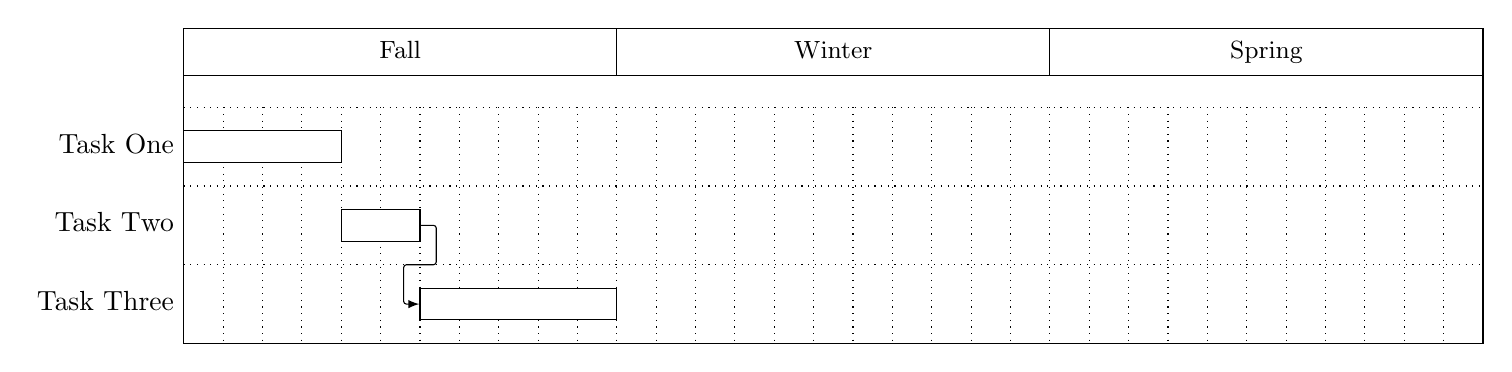
\begin{tikzpicture}[x=.5cm, y=2cm]
\begin{ganttchart}[vgrid, hgrid]{1}{33} % 3 terms
\gantttitle{Fall}{11} \gantttitle{Winter}{11} \gantttitle{Spring}{11} \\
\ganttbar{Task One}{1}{4} \\    
\ganttbar[name=b2]{Task Two}{5}{6} \\      
\ganttbar[name=b3]{Task Three}{7}{11}
\ganttlink{b2}{b3}
\end{ganttchart}
\end{tikzpicture}
}

\end{document}
